% Options for packages loaded elsewhere
\PassOptionsToPackage{unicode}{hyperref}
\PassOptionsToPackage{hyphens}{url}
\PassOptionsToPackage{space}{xeCJK}
\documentclass[
  10pt,
  a4paper,
]{article}
\usepackage{xcolor}
\usepackage[margin=22mm]{geometry}
\usepackage{pdflscape}
\usepackage{amsmath,amssymb}
\setcounter{secnumdepth}{-\maxdimen} % remove section numbering
\usepackage{iftex}
\ifPDFTeX
  \usepackage[T1]{fontenc}
  \usepackage[utf8]{inputenc}
  \usepackage{textcomp} % provide euro and other symbols
\else % if luatex or xetex
  \usepackage{unicode-math} % this also loads fontspec
  \defaultfontfeatures{Scale=MatchLowercase}
  \defaultfontfeatures[\rmfamily]{Ligatures=TeX,Scale=1}
\fi
\usepackage{lmodern}
\ifPDFTeX\else
  % xetex/luatex font selection
  \ifXeTeX
    \usepackage{xeCJK}
    \setCJKmainfont[]{Hiragino Mincho ProN}
  \fi
  \ifLuaTeX
    \usepackage[]{luatexja-fontspec}
    \setmainjfont[]{Hiragino Mincho ProN}
  \fi
\fi
% Use upquote if available, for straight quotes in verbatim environments
\IfFileExists{upquote.sty}{\usepackage{upquote}}{}
\IfFileExists{microtype.sty}{% use microtype if available
  \usepackage[]{microtype}
  \UseMicrotypeSet[protrusion]{basicmath} % disable protrusion for tt fonts
}{}
\makeatletter
\@ifundefined{KOMAClassName}{% if non-KOMA class
  \IfFileExists{parskip.sty}{%
    \usepackage{parskip}
  }{% else
    \setlength{\parindent}{0pt}
    \setlength{\parskip}{6pt plus 2pt minus 1pt}}
}{% if KOMA class
  \KOMAoptions{parskip=half}}
\makeatother
\usepackage{color}
\usepackage{fancyvrb}
\newcommand{\VerbBar}{|}
\newcommand{\VERB}{\Verb[commandchars=\\\{\}]}
\DefineVerbatimEnvironment{Highlighting}{Verbatim}{commandchars=\\\{\}}
% Add ',fontsize=\small' for more characters per line
\newenvironment{Shaded}{}{}
\newcommand{\AlertTok}[1]{\textcolor[rgb]{1.00,0.00,0.00}{\textbf{#1}}}
\newcommand{\AnnotationTok}[1]{\textcolor[rgb]{0.38,0.63,0.69}{\textbf{\textit{#1}}}}
\newcommand{\AttributeTok}[1]{\textcolor[rgb]{0.49,0.56,0.16}{#1}}
\newcommand{\BaseNTok}[1]{\textcolor[rgb]{0.25,0.63,0.44}{#1}}
\newcommand{\BuiltInTok}[1]{\textcolor[rgb]{0.00,0.50,0.00}{#1}}
\newcommand{\CharTok}[1]{\textcolor[rgb]{0.25,0.44,0.63}{#1}}
\newcommand{\CommentTok}[1]{\textcolor[rgb]{0.38,0.63,0.69}{\textit{#1}}}
\newcommand{\CommentVarTok}[1]{\textcolor[rgb]{0.38,0.63,0.69}{\textbf{\textit{#1}}}}
\newcommand{\ConstantTok}[1]{\textcolor[rgb]{0.53,0.00,0.00}{#1}}
\newcommand{\ControlFlowTok}[1]{\textcolor[rgb]{0.00,0.44,0.13}{\textbf{#1}}}
\newcommand{\DataTypeTok}[1]{\textcolor[rgb]{0.56,0.13,0.00}{#1}}
\newcommand{\DecValTok}[1]{\textcolor[rgb]{0.25,0.63,0.44}{#1}}
\newcommand{\DocumentationTok}[1]{\textcolor[rgb]{0.73,0.13,0.13}{\textit{#1}}}
\newcommand{\ErrorTok}[1]{\textcolor[rgb]{1.00,0.00,0.00}{\textbf{#1}}}
\newcommand{\ExtensionTok}[1]{#1}
\newcommand{\FloatTok}[1]{\textcolor[rgb]{0.25,0.63,0.44}{#1}}
\newcommand{\FunctionTok}[1]{\textcolor[rgb]{0.02,0.16,0.49}{#1}}
\newcommand{\ImportTok}[1]{\textcolor[rgb]{0.00,0.50,0.00}{\textbf{#1}}}
\newcommand{\InformationTok}[1]{\textcolor[rgb]{0.38,0.63,0.69}{\textbf{\textit{#1}}}}
\newcommand{\KeywordTok}[1]{\textcolor[rgb]{0.00,0.44,0.13}{\textbf{#1}}}
\newcommand{\NormalTok}[1]{#1}
\newcommand{\OperatorTok}[1]{\textcolor[rgb]{0.40,0.40,0.40}{#1}}
\newcommand{\OtherTok}[1]{\textcolor[rgb]{0.00,0.44,0.13}{#1}}
\newcommand{\PreprocessorTok}[1]{\textcolor[rgb]{0.74,0.48,0.00}{#1}}
\newcommand{\RegionMarkerTok}[1]{#1}
\newcommand{\SpecialCharTok}[1]{\textcolor[rgb]{0.25,0.44,0.63}{#1}}
\newcommand{\SpecialStringTok}[1]{\textcolor[rgb]{0.73,0.40,0.53}{#1}}
\newcommand{\StringTok}[1]{\textcolor[rgb]{0.25,0.44,0.63}{#1}}
\newcommand{\VariableTok}[1]{\textcolor[rgb]{0.10,0.09,0.49}{#1}}
\newcommand{\VerbatimStringTok}[1]{\textcolor[rgb]{0.25,0.44,0.63}{#1}}
\newcommand{\WarningTok}[1]{\textcolor[rgb]{0.38,0.63,0.69}{\textbf{\textit{#1}}}}
\usepackage{longtable,booktabs,array}
\newcounter{none} % for unnumbered tables
\usepackage{calc} % for calculating minipage widths
% Correct order of tables after \paragraph or \subparagraph
\usepackage{etoolbox}
\makeatletter
\patchcmd\longtable{\par}{\if@noskipsec\mbox{}\fi\par}{}{}
\makeatother
% Allow footnotes in longtable head/foot
\IfFileExists{footnotehyper.sty}{\usepackage{footnotehyper}}{\usepackage{footnote}}
\makesavenoteenv{longtable}
\usepackage{graphicx}
\makeatletter
\newsavebox\pandoc@box
\newcommand*\pandocbounded[1]{% scales image to fit in text height/width
  \sbox\pandoc@box{#1}%
  \Gscale@div\@tempa{\textheight}{\dimexpr\ht\pandoc@box+\dp\pandoc@box\relax}%
  \Gscale@div\@tempb{\linewidth}{\wd\pandoc@box}%
  \ifdim\@tempb\p@<\@tempa\p@\let\@tempa\@tempb\fi% select the smaller of both
  \ifdim\@tempa\p@<\p@\scalebox{\@tempa}{\usebox\pandoc@box}%
  \else\usebox{\pandoc@box}%
  \fi%
}
% Set default figure placement to htbp
\def\fps@figure{htbp}
\makeatother
\setlength{\emergencystretch}{3em} % prevent overfull lines
\providecommand{\tightlist}{%
  \setlength{\itemsep}{0pt}\setlength{\parskip}{0pt}}
\usepackage{bookmark}
\IfFileExists{xurl.sty}{\usepackage{xurl}}{} % add URL line breaks if available
\urlstyle{same}
\hypersetup{
  hidelinks,
  pdfcreator={LaTeX via pandoc}}

\author{}
\date{}

\begin{document}

\section{An Inverse-Square Law from a Future-Phase-Position Acceleration
Map and Harmonic Closure in a Closed Two-Body AB Phase
System}\label{an-inverse-square-law-from-a-future-phase-position-acceleration-map-and-harmonic-closure-in-a-closed-two-body-ab-phase-system}

\subsection{Reanalysis of the Published Acceleration Experiment and
Derivation of the Distance Exponent with Respect to Phase-Cell
Width}\label{reanalysis-of-the-published-acceleration-experiment-and-derivation-of-the-distance-exponent-with-respect-to-phase-cell-width}

\textbf{Author:} Noriaki Kihara\\
\textbf{Affiliation:} WF System Co., Ltd.\\
\textbf{ORCID:} 0009-0004-6753-4020\\
\textbf{Date:} July 19, 2026\\
\textbf{Version DOI:} 10.5281/zenodo.21441082\\
\textbf{Concept DOI:} 10.5281/zenodo.21441081\\
\textbf{Position in series:} Wave Information Readout series;
supplementary paper v1 for the two-body AB acceleration experiment

\begin{center}\rule{0.5\linewidth}{0.5pt}\end{center}

\subsection{Abstract}\label{abstract}

In a preceding numerical experiment on a closed two-body AB phase
system, an acceleration-like harmonic readout with a nonzero second
difference in relative positional phase was obtained solely from the
unlabeled two-body relation \(f_{AB}\), without introducing a standard
external force, background space, gravitational equation, or Coulomb
equation. The readout was not, however, found to be inversely
proportional or inverse-square proportional to distance. In a subsequent
ABC experiment that introduced an independent metric wave \(C\), the
principal readout also remained proportional.

This paper reexamines why the inverse-square dependence was not
detected. The preceding experiment varied the initial positional-phase
deviation as an amplitude while holding the harmonic period fixed. Its
native acceleration-like readout was therefore proportional to the
amplitude. The ABC experiment also inherited the basic relation
\(f_{AB}=L_{AB}\), and the observation wave \(C\) did not change its
exponent. Those experiments consequently tested whether changing an
amplitude or readout distance would automatically generate an inverse
square; they did not test the relation between a closed phase-cell width
and the harmonic angular speed belonging to that cell.

Here, a future phase position seen from the present position on a closed
orbit is defined as a relational rotation center. The existing
centripetal closure compensation is read as acceleration in the
tangential direction through the map

\[
\alpha=R\omega^2.
\]

For every nonzero integer harmonic \(n\), we further read

\[
\Delta\theta_n=\frac{2\pi}{|n|},
\qquad
\omega_n=n\omega_1
\]

as one harmonic closure condition. It follows that

\[
|\omega_n|\Delta\theta_n
=2\pi\omega_1
\equiv\Omega,
\]

so the angular speed and phase-cell width cannot be chosen
independently. Connecting this closure condition to the acceleration
relation already confirmed in the experiment gives

\[
\alpha_n
=R|\omega_n|^2
=\frac{R\Omega^2}{\Delta\theta_n^2}.
\]

Under the specific conditions of the reported experiment, the
inverse-square law was established. No new reciprocal term,
area-dilution term, spherical shell, external force, or gravitational
constant is introduced.

What remains untested is whether the mechanism generalizes to arbitrary
closed systems, arbitrary harmonic arrangements, arbitrary nonharmonic
updates, or arbitrary distance readouts. The principal result is that,
under the conditions of the published AB experiment, the
acceleration-like second-order structure becomes an inverse-square law
with respect to phase-cell width when it is connected to harmonic
closure within the same phase system.

\begin{center}\rule{0.5\linewidth}{0.5pt}\end{center}

\subsection{0. Conclusion}\label{conclusion}

The conclusion of this paper is as follows.

The published two-body AB experiment had already produced a nonzero
acceleration-like second-order structure from the unlabeled two-body
relation \(f_{AB}\) alone.

The inverse square did not appear in that experiment because the
positional-phase deviation was varied as an amplitude while the harmonic
period was held fixed.

In the present reanalysis, a future phase position on the closed orbit
is read as a relational rotation center, and the acceleration relation

\[
\alpha=R\omega^2
\]

is connected to the harmonic closure

\[
|\omega_n|\Delta\theta_n=\Omega.
\]

As a result, under the specific conditions of this experiment,

\[
\alpha_n
=\frac{R\Omega^2}{\Delta\theta_n^2}
\]

is an inverse-square law.

This result was not obtained by adding \(1/L^2\) to the existing
experiment.

The inverse square is produced by the simultaneous validity of two
conditions:

\begin{enumerate}
\def\labelenumi{\arabic{enumi}.}
\tightlist
\item
  the acceleration map centered on a future phase position,
\end{enumerate}

\[
\alpha_n=R|\omega_n|^2,
\]

\begin{enumerate}
\def\labelenumi{\arabic{enumi}.}
\setcounter{enumi}{1}
\tightlist
\item
  the relation between harmonic number and phase-cell width on a closed
  phase circle,
\end{enumerate}

\[
|\omega_n|\Delta\theta_n=\Omega.
\]

Connecting the two gives

\[
\boxed{
\alpha_n
=\frac{R\Omega^2}{\Delta\theta_n^2}
}.
\]

This paper does not derive gravity.

It identifies a mechanism by which an acceleration-like second-order
structure in a closed phase system without a preassigned background
coordinate system is read as an inverse-square law with respect to
phase-cell width.

\begin{center}\rule{0.5\linewidth}{0.5pt}\end{center}

\subsection{1. Research Question}\label{research-question}

\subsubsection{1.1 What had been established in the preceding AB
experiment}\label{what-had-been-established-in-the-preceding-ab-experiment}

The preceding experiment on a closed two-body AB phase system
established the following:

\begin{quote}
An acceleration-like harmonic readout can be obtained from the closed
phase relation between A and B alone.
\end{quote}

None of the following equations was introduced externally:

\[
\begin{aligned}
F&=ma,\\
F&=-kx,\\
F&=\frac{Gm_A m_B}{L_{AB}^2},\\
F&=\frac{q_Aq_B}{4\pi\varepsilon_0L_{AB}^2}.
\end{aligned}
\]

Nor were individual forces \(f_A\) and \(f_B\) introduced.

The experiment used only the unlabeled relation \(f_{AB}\) between A and
B.

\subsubsection{1.2 What remained
unresolved}\label{what-remained-unresolved}

The preceding AB paper recorded the following boundary concerning the
distance exponent:

\begin{quote}
From the two-body AB system alone, it was not possible to determine
whether the acceleration-like readout changed inversely or
inverse-square proportionally to the positional-phase difference, that
is, to distance.
\end{quote}

A subsequent ABC experiment introduced a third wave \(C\) as an
independent metric gauge. The principal classification in the
gauge-effective cases was nevertheless

\[
I_{AB}(L)\propto L,
\]

and neither an inverse nor an inverse-square form appeared.

\subsubsection{1.3 Question addressed
here}\label{question-addressed-here}

The question is not whether an inverse square appears after adding a
third wave or a new spatial dimension.

The question is:

\begin{quote}
What distance exponent results when the acceleration-like second-order
structure already obtained in the preceding AB experiment is reread
through the relation between harmonics and phase-cell width on a closed
phase circle?
\end{quote}

\begin{center}\rule{0.5\linewidth}{0.5pt}\end{center}

\subsection{2. Classification of Claims}\label{classification-of-claims}

{\def\LTcaptype{none} % do not increment counter
\begin{longtable}[]{@{}
  >{\raggedright\arraybackslash}p{(\linewidth - 4\tabcolsep) * \real{0.3333}}
  >{\raggedright\arraybackslash}p{(\linewidth - 4\tabcolsep) * \real{0.3333}}
  >{\raggedright\arraybackslash}p{(\linewidth - 4\tabcolsep) * \real{0.3333}}@{}}
\toprule\noalign{}
\begin{minipage}[b]{\linewidth}\raggedright
Subject
\end{minipage} & \begin{minipage}[b]{\linewidth}\raggedright
Classification
\end{minipage} & \begin{minipage}[b]{\linewidth}\raggedright
Basis
\end{minipage} \\
\midrule\noalign{}
\endhead
\bottomrule\noalign{}
\endlastfoot
A nonzero second difference exists in the AB experiment & Existing
numerical fact & Recomputed from the published CSV data \\
\(\Delta^2\chi_s=-\omega_d^2\chi_s\) & Derived consequence, numerically
verified & Regression slope agrees with theory in all eight
conditions \\
Preservation of \(Q_{\mathrm{closed}}=0\) & Existing numerical fact &
Maximum residual is zero in all eight conditions \\
A future phase position is treated as a relational rotation center &
Physical interpretation & Maps the existing centripetal compensation
into the tangential direction \\
\(\alpha=R\omega^2\) & Definition of acceleration map & Defined from the
radius and angular speed of the virtual rotation \\
\(\Delta\theta_n=2\pi/\lvert n\rvert\) & Definition of harmonic closure
& One cycle is closed by \(\lvert n\rvert\) identical phase cells \\
\(\omega_n=n\omega_1\) & Harmonic condition & Integer harmonic of the
fundamental angular speed \\
\(\lvert\omega_n\rvert\Delta\theta_n=\Omega\) & Derived consequence &
Product of the preceding two equations \\
\(\alpha_n=R\Omega^2/\Delta\theta_n^2\) & Derived consequence &
Algebraic connection of the acceleration map and harmonic closure \\
The inverse-square law holds under the tested conditions & Principal
result & Connection to the existing acceleration experiment \\
The same mechanism holds in every closed system & Untested & The paper
addresses the existing AB experimental conditions \\
The acceleration is identical to standard gravity & Not derived & No
gravitational constant, mass source, or field equation is introduced \\
\end{longtable}
}

\begin{center}\rule{0.5\linewidth}{0.5pt}\end{center}

\subsection{3. Why the Previous Experiment Did Not Produce an Inverse
Square}\label{why-the-previous-experiment-did-not-produce-an-inverse-square}

\subsubsection{3.1 Quantity varied in the AB inverse-area
experiment}\label{quantity-varied-in-the-ab-inverse-area-experiment}

In the preceding AB inverse-area extension sweep, the initial
positional-phase deviation was denoted by \(\delta\), and the experiment
used

\[
\chi_s
=\delta\lambda_s\cos(\omega_{\mathrm{step}}s),
\]

\[
\tau_s
=\delta A_\tau\lambda_s
\sin(r_\tau\omega_{\mathrm{step}}s+\phi_\tau).
\]

The value of \(\delta\) was varied, whereas the fundamental update angle
of the spatial phase was fixed at

\[
\omega_{\mathrm{step}}
=\frac{2\pi}{96}.
\]

The native AB acceleration candidate was calculated as

\[
f_{AB}^{\mathrm{native}}
=\omega_d^2\max|\chi|,
\]

with

\[
\omega_d^2
=4\sin^2\left(\frac{\pi}{96}\right).
\]

At fixed \(\omega_d\), therefore,

\[
f_{AB}^{\mathrm{native}}\propto\delta.
\]

This is a proportional form.

Meanwhile, the area spanned by \(\chi\) and \(\tau\) is

\[
A_{\chi\tau}\propto\delta^2.
\]

One can consequently construct

\[
\frac{1}{A_{\chi\tau}}
\]

in postprocessing and obtain

\[
\frac{1}{A_{\chi\tau}}
\propto\frac{1}{\delta^2}.
\]

That quantity was a constructed control, however, not a native readout.

The result of the preceding experiment was correct. Because it treated
the amplitude \(\delta\) and harmonic angular speed \(\omega\) as
independent, the native quantity was proportional.

\subsubsection{3.2 Why the ABC independent-metric experiment was
proportional}\label{why-the-abc-independent-metric-experiment-was-proportional}

The subsequent ABC experiment inherited the basic AB relation

\[
f_{AB}=L_{AB}.
\]

Its principal candidate for a \(C\)-based acceleration readout was

\[
a_{AB}^{(C)}
=\left|L_{AB}^{(C)}+f_{AC}-f_{BC}\right|.
\]

For a symmetric placement of \(C\), the difference \(f_{AC}-f_{BC}\)
vanishes, and therefore

\[
a_{AB}^{(C)}\propto L_{AB}^{(C)}.
\]

The proportional result of the ABC experiment thus agrees with its
implementation.

The third wave \(C\) acts as a metric gauge that reads the AB distance.
Adding a metric gauge alone does not change the distance exponent of the
basic relation.

\subsubsection{3.3 Quantity reconsidered in this
paper}\label{quantity-reconsidered-in-this-paper}

The preceding experiments varied:

\begin{Shaded}
\begin{Highlighting}[]
\NormalTok{initial positional{-}phase deviation}
\NormalTok{amplitude ratio}
\NormalTok{frequency ratio of the temporal phase}
\NormalTok{temporal phase difference}
\NormalTok{readout damping}
\NormalTok{C{-}gauge strength}
\NormalTok{C{-}gauge arrangement}
\end{Highlighting}
\end{Shaded}

The independent variable considered here is different. We read the
integer harmonic \(n\) constituting a closed phase circle and the width
of one phase cell fixed by that harmonic,

\[
\Delta\theta_n=\frac{2\pi}{|n|}.
\]

When \(\Delta\theta_n\) is varied, \(\omega\) must not be held fixed.
The same integer harmonic simultaneously determines

\[
\omega_n=n\omega_1.
\]

The inverse square does not arise from amplitude dilution. It arises
because the harmonic angular speed and the phase-cell width share the
same closure integer \(n\).

\begin{center}\rule{0.5\linewidth}{0.5pt}\end{center}

\subsection{4. Reconfirmation of the Published AB Acceleration
Experiment}\label{reconfirmation-of-the-published-ab-acceleration-experiment}

\subsubsection{4.1 Data source}\label{data-source}

This paper reuses the following published experimental results:

\begin{Shaded}
\begin{Highlighting}[]
\NormalTok{波の情報読出し/20260711/}
\NormalTok{ab\_two\_body\_fermionic\_reflection\_harmonic\_readout\_preliminary\_result\_v4/}
\end{Highlighting}
\end{Shaded}

No new motion update, scattering calculation, or parameter sweep is
performed.

The eight target conditions are:

\begin{Shaded}
\begin{Highlighting}[]
\NormalTok{initial deviations: 2 degrees, 5 degrees, 10 degrees, 20 degrees}
\NormalTok{protocols: transmission and fermionic reflection}
\end{Highlighting}
\end{Shaded}

\subsubsection{4.2 Acceleration-like second-order
structure}\label{acceleration-like-second-order-structure}

Let the stored relative positional phase be \(\chi_s\). Define its
discrete second difference by

\[
\Delta^2\chi_s
=\chi_{s+1}-2\chi_s+\chi_{s-1}.
\]

In all eight conditions,

\[
\Delta^2\chi_s
=-\omega_d^2\chi_s
\]

was satisfied.

For a period of 96 steps, the discrete coefficient is

\[
\omega_d^2
=4\sin^2\left(\frac{\pi}{96}\right)
=0.0042821535227929855.
\]

\subsubsection{4.3 Aggregate results}\label{aggregate-results}

\begin{landscape}
{\def\LTcaptype{none} % do not increment counter
\begin{longtable}[]{@{}
  >{\raggedleft\arraybackslash}p{(\linewidth - 14\tabcolsep) * \real{0.1290}}
  >{\raggedright\arraybackslash}p{(\linewidth - 14\tabcolsep) * \real{0.0968}}
  >{\raggedleft\arraybackslash}p{(\linewidth - 14\tabcolsep) * \real{0.1290}}
  >{\raggedleft\arraybackslash}p{(\linewidth - 14\tabcolsep) * \real{0.1290}}
  >{\raggedleft\arraybackslash}p{(\linewidth - 14\tabcolsep) * \real{0.1290}}
  >{\raggedleft\arraybackslash}p{(\linewidth - 14\tabcolsep) * \real{0.1290}}
  >{\raggedleft\arraybackslash}p{(\linewidth - 14\tabcolsep) * \real{0.1290}}
  >{\raggedleft\arraybackslash}p{(\linewidth - 14\tabcolsep) * \real{0.1290}}@{}}
\toprule\noalign{}
\begin{minipage}[b]{\linewidth}\raggedleft
Initial deviation
\end{minipage} & \begin{minipage}[b]{\linewidth}\raggedright
Protocol
\end{minipage} & \begin{minipage}[b]{\linewidth}\raggedleft
Maximum \(\lvert\Delta^2\chi\rvert\)
\end{minipage} & \begin{minipage}[b]{\linewidth}\raggedleft
Regression slope
\end{minipage} & \begin{minipage}[b]{\linewidth}\raggedleft
Theoretical slope
\end{minipage} & \begin{minipage}[b]{\linewidth}\raggedleft
\(R^2\)
\end{minipage} & \begin{minipage}[b]{\linewidth}\raggedleft
Maximum displayed difference
\end{minipage} & \begin{minipage}[b]{\linewidth}\raggedleft
\(\max\lvert Q_{\mathrm{closed}}\rvert\)
\end{minipage} \\
\midrule\noalign{}
\endhead
\bottomrule\noalign{}
\endlastfoot
2 degrees & Transmission & \(1.494753561\times10^{-4}\) &
\(-4.282153522793\times10^{-3}\) & \(-4.282153522793\times10^{-3}\) &
1.000000000000 & \(2.479\times10^{-16}\) & 0 \\
2 degrees & Fermionic reflection & \(1.494753561\times10^{-4}\) &
\(-4.282153522793\times10^{-3}\) & \(-4.282153522793\times10^{-3}\) &
1.000000000000 & \(2.475\times10^{-16}\) & 0 \\
5 degrees & Transmission & \(3.736883902\times10^{-4}\) &
\(-4.282153522793\times10^{-3}\) & \(-4.282153522793\times10^{-3}\) &
1.000000000000 & \(6.201\times10^{-16}\) & 0 \\
5 degrees & Fermionic reflection & \(3.736883902\times10^{-4}\) &
\(-4.282153522793\times10^{-3}\) & \(-4.282153522793\times10^{-3}\) &
1.000000000000 & \(6.219\times10^{-16}\) & 0 \\
10 degrees & Transmission & \(7.473767805\times10^{-4}\) &
\(-4.282153522793\times10^{-3}\) & \(-4.282153522793\times10^{-3}\) &
1.000000000000 & \(1.240\times10^{-15}\) & 0 \\
10 degrees & Fermionic reflection & \(7.473767805\times10^{-4}\) &
\(-4.282153522793\times10^{-3}\) & \(-4.282153522793\times10^{-3}\) &
1.000000000000 & \(1.244\times10^{-15}\) & 0 \\
20 degrees & Transmission & \(1.494753561\times10^{-3}\) &
\(-4.282153522793\times10^{-3}\) & \(-4.282153522793\times10^{-3}\) &
1.000000000000 & \(2.481\times10^{-15}\) & 0 \\
20 degrees & Fermionic reflection & \(1.494753561\times10^{-3}\) &
\(-4.282153522793\times10^{-3}\) & \(-4.282153522793\times10^{-3}\) &
1.000000000000 & \(2.488\times10^{-15}\) & 0 \\
\end{longtable}
}
\end{landscape}

The regression slope agrees with the theoretical value in all eight
conditions.

The transmission and fermionic-reflection protocols reduce to the same
second-order relation. In addition,

\[
Q_{\mathrm{closed}}=0
\]

is preserved in all conditions.

\subsubsection{4.4 Figure}\label{figure}

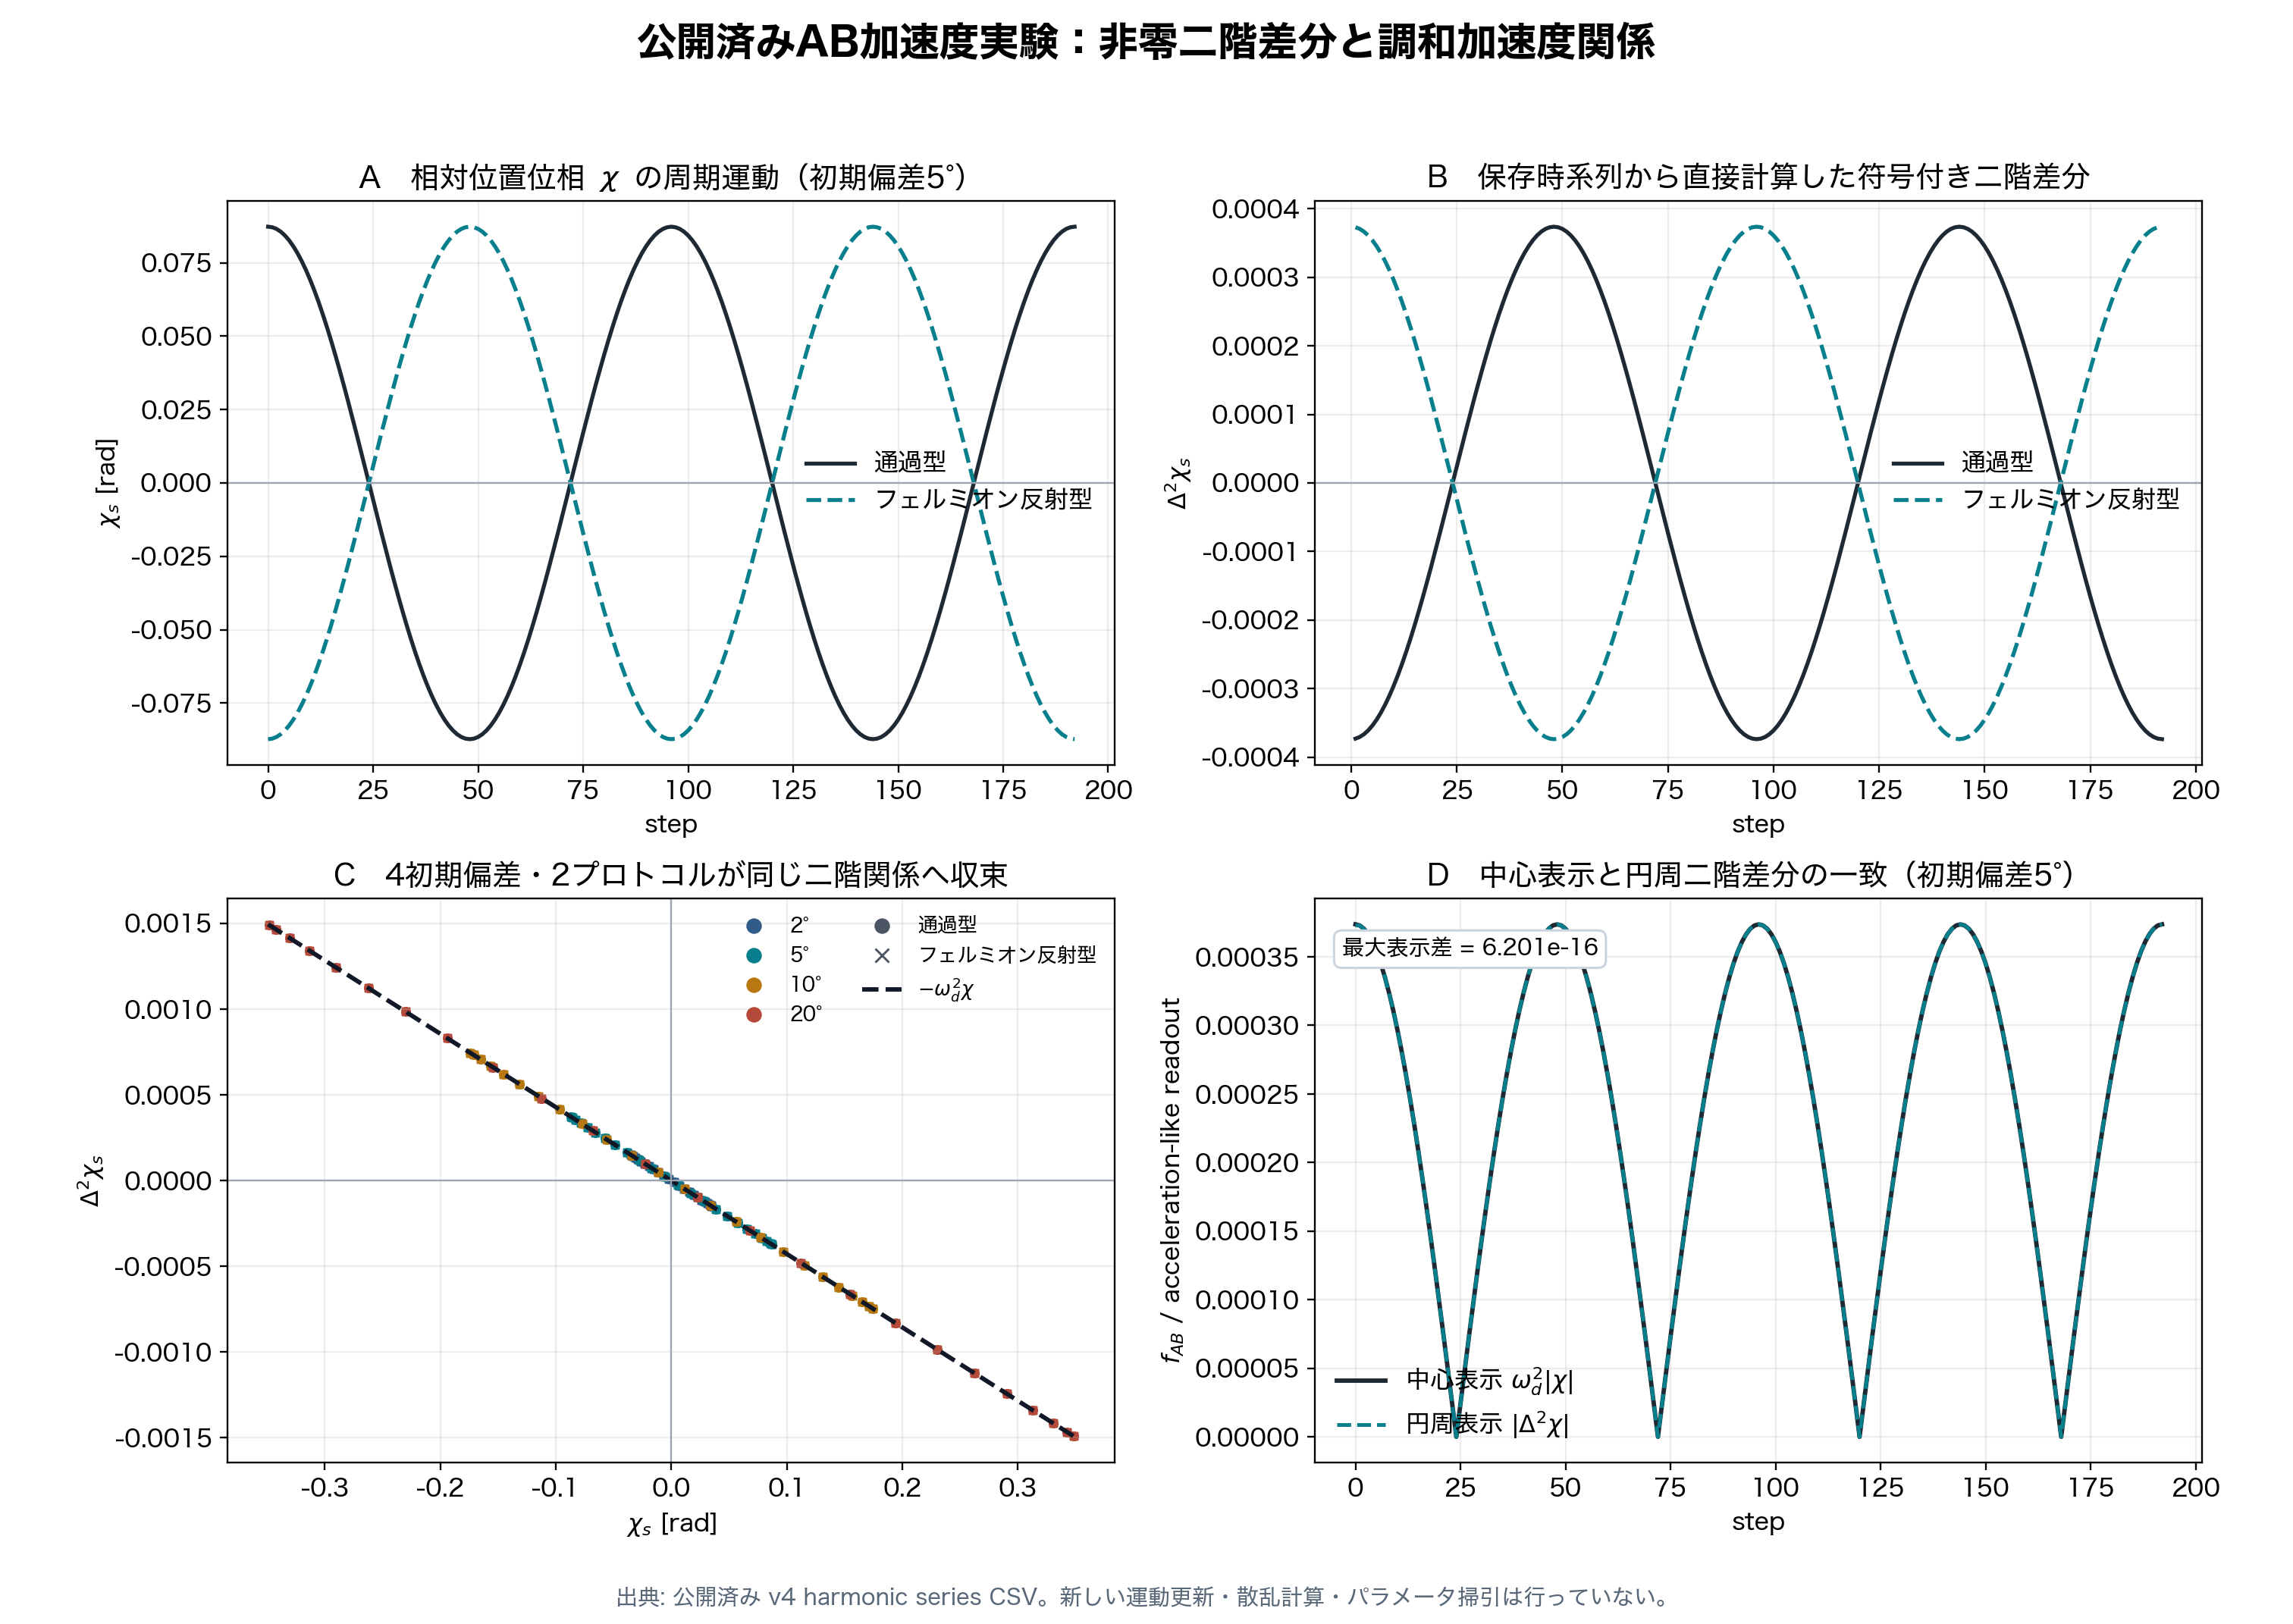
\includegraphics[width=0.95\linewidth,height=\textheight,keepaspectratio]{figures/既存AB加速度時系列と二階差分整合_v1.png}

Panel A shows the periodic motion of the relative positional phase
\(\chi_s\). Panel B shows the signed second difference calculated
directly from the stored time series.

Panel C shows that every point in the four initial deviations and two
protocols lies on

\[
\Delta^2\chi_s=-\omega_d^2\chi_s.
\]

Panel D shows that the centripetal representation \(\omega_d^2|\chi|\)
agrees with the tangential readout \(|\Delta^2\chi|\), with a maximum
displayed difference of \(6.201\times10^{-16}\).

Thus, the acceleration-like second-order structure connected in this
paper is not a newly assumed quantity; it is an observable already
present in the published data.

\begin{center}\rule{0.5\linewidth}{0.5pt}\end{center}

\subsection{5. Acceleration Map Centered on a Future Phase
Position}\label{acceleration-map-centered-on-a-future-phase-position}

\subsubsection{5.1 Reading a relational future position rather than a
fixed
center}\label{reading-a-relational-future-position-rather-than-a-fixed-center}

In the preceding experiment, \(f_{AB}\) was displayed as centripetal
compensation closing the AB relation.

Here, the center is not treated as a fixed point in an external space.

Let \(P\) be the present phase position on the closed orbit,
\(\hat{\boldsymbol t}\) the unit vector in the direction of phase
progression, and \(R\) the relational radius of curvature. Define the
future-phase-position center \(C_f\) by

\[
\boldsymbol C_f
=\boldsymbol P+R\hat{\boldsymbol t}.
\]

\(C_f\) is not a fixed center placed a priori in a background space. It
is defined at each position from the relation among the present
position, the direction of phase progression, and the closure radius.

\subsubsection{5.2 Acceleration map}\label{acceleration-map}

Define a virtual rotation of angular speed \(\omega\) around \(C_f\).
Its center-directed acceleration vector is

\[
\boldsymbol\alpha(P)
=\omega^2(\boldsymbol C_f-\boldsymbol P).
\]

By definition,

\[
\boldsymbol C_f-\boldsymbol P
=R\hat{\boldsymbol t},
\]

and therefore

\[
\boldsymbol\alpha(P)
=R\omega^2\hat{\boldsymbol t}.
\]

Its magnitude is

\[
\boxed{
\alpha=R\omega^2
}.
\]

No new force is added. The same \(f_{AB}\) retained as centripetal
compensation in the preceding experiment is mapped into the tangential
direction defined by the future phase position.

\subsubsection{5.3 Diagram}\label{diagram}

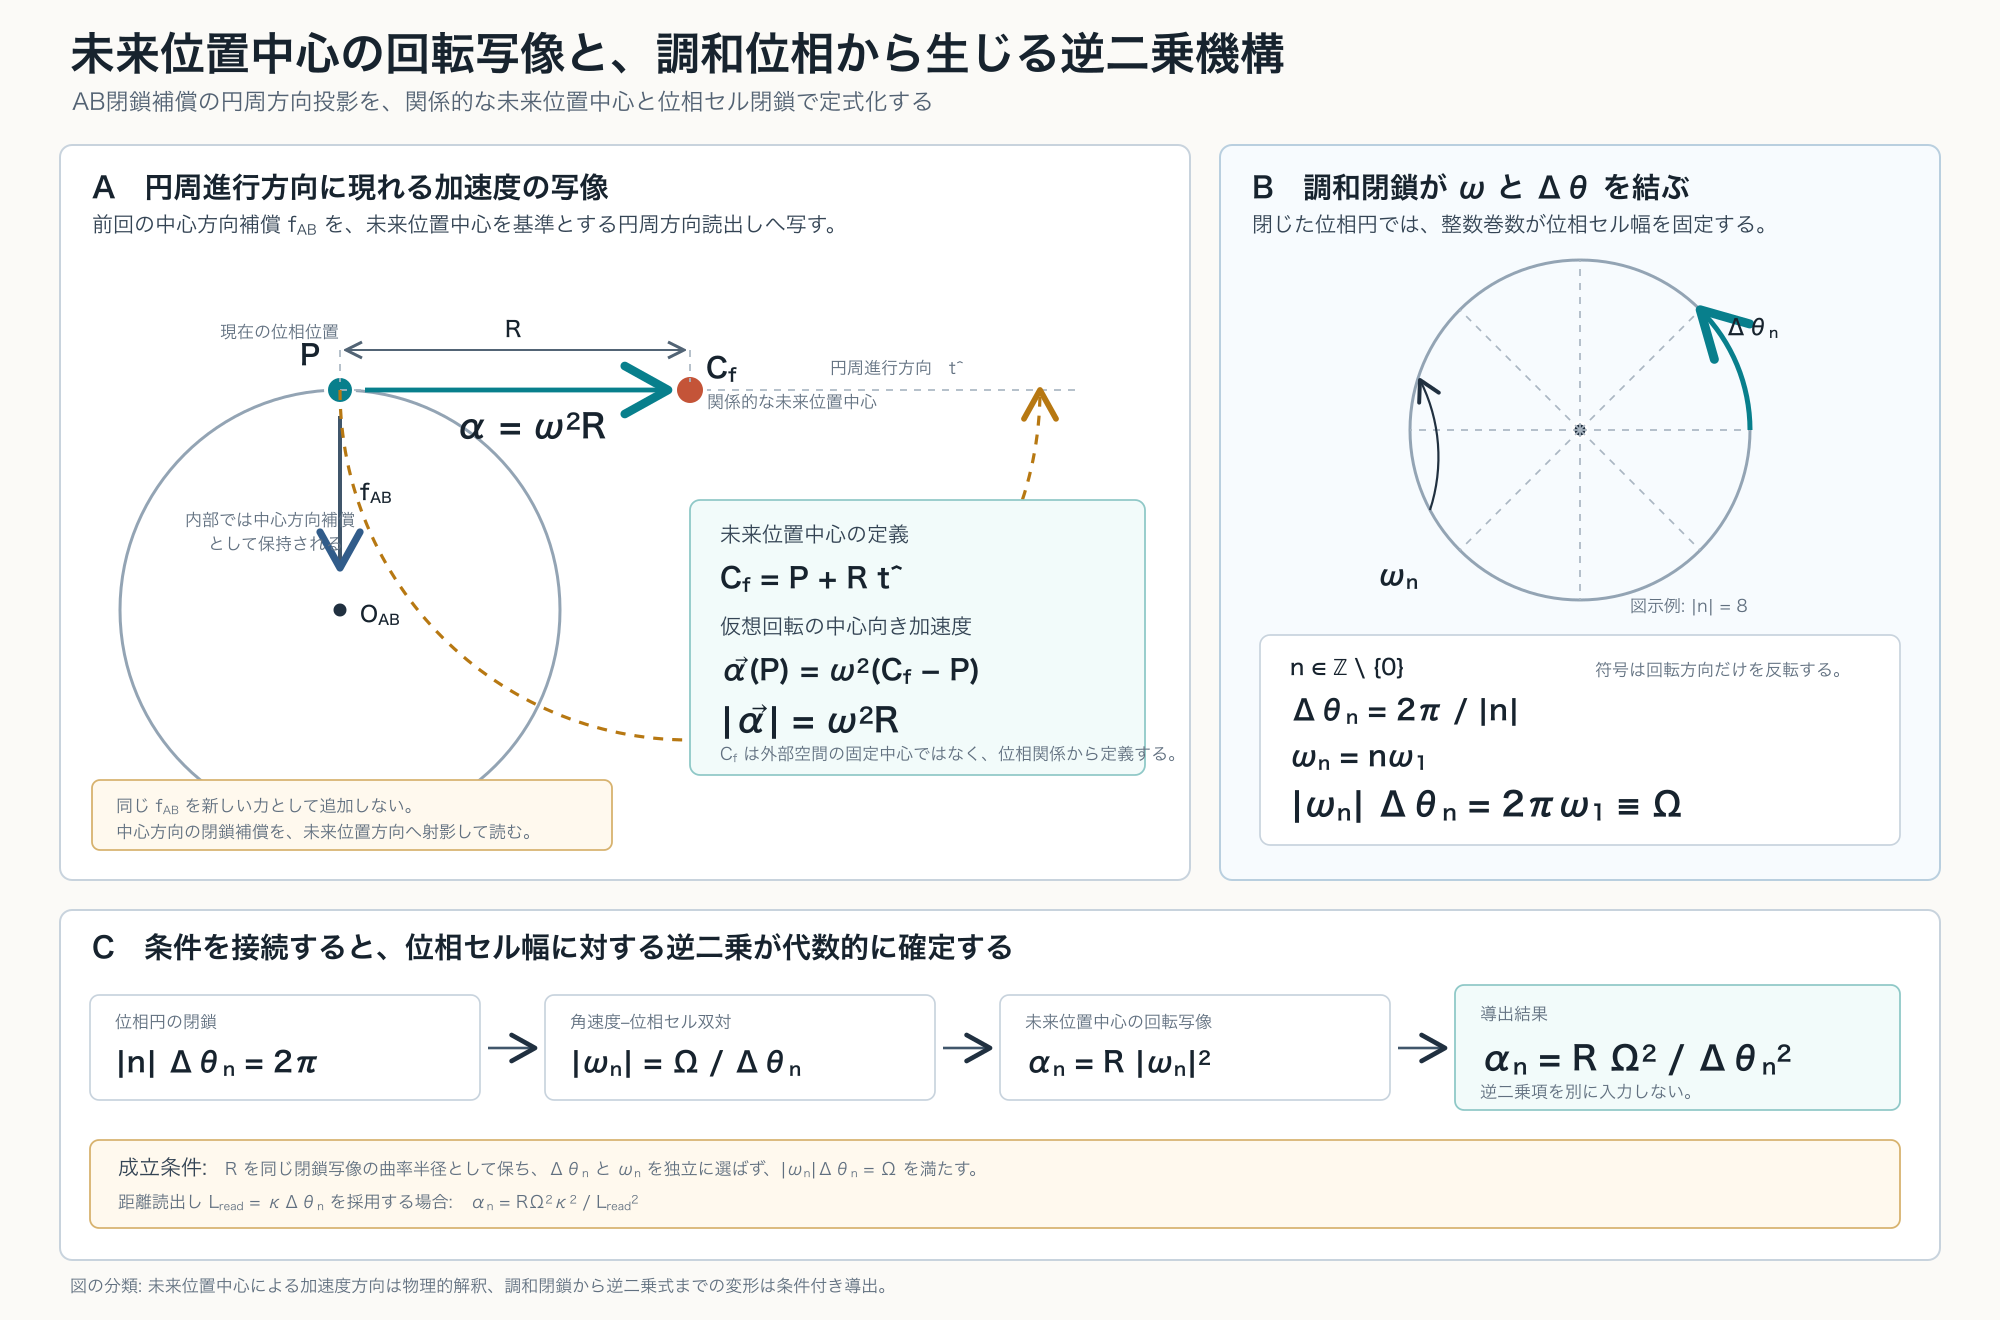
\includegraphics[width=0.95\linewidth,height=\textheight,keepaspectratio]{figures/未来位置中心回転写像と調和位相逆二乗機構_v1.png}

Panel A maps the centripetal compensation of the preceding experiment to
tangential acceleration around the future-phase-position center.

Panel B shows that an integer harmonic simultaneously fixes the
phase-cell width and angular speed.

Panel C shows that connecting these two conditions yields the
inverse-square law.

\begin{center}\rule{0.5\linewidth}{0.5pt}\end{center}

\subsection{6. Harmonic Closure Connects Angular Speed and Phase-Cell
Width}\label{harmonic-closure-connects-angular-speed-and-phase-cell-width}

\subsubsection{6.1 Nonzero integer
harmonics}\label{nonzero-integer-harmonics}

Let one complete phase circle be partitioned into \(|n|\) equal phase
cells, where

\[
n\in\mathbb Z\setminus\{0\}.
\]

The case \(n=0\) creates no nonzero cell that partitions a complete
cycle and carries no phase progression; it is excluded from the
acceleration readout considered here.

The width of one phase cell is

\[
\boxed{
\Delta\theta_n
=\frac{2\pi}{|n|}
}.
\]

\subsubsection{6.2 Harmonic angular speed}\label{harmonic-angular-speed}

Let the fundamental angular speed be \(\omega_1\). The angular speed of
the \(n\)th harmonic is

\[
\boxed{
\omega_n=n\omega_1
}.
\]

The sign of \(n\) represents the orientation of phase rotation; the
magnitude of the acceleration depends on \(|n|\).

\subsubsection{6.3 Dual relation between angular speed and phase-cell
width}\label{dual-relation-between-angular-speed-and-phase-cell-width}

Multiplying the two equations gives

\[
|\omega_n|\Delta\theta_n
=|n|\omega_1\frac{2\pi}{|n|}
=2\pi\omega_1.
\]

Define

\[
\Omega\equiv2\pi\omega_1.
\]

Then

\[
\boxed{
|\omega_n|\Delta\theta_n=\Omega
},
\]

and hence

\[
\boxed{
|\omega_n|
=\frac{\Omega}{\Delta\theta_n}
}.
\]

This is not a reciprocal law imposed from outside. It is the algebraic
consequence of the phase-circle closure condition and integer-harmonic
condition sharing the same integer \(n\).

\begin{center}\rule{0.5\linewidth}{0.5pt}\end{center}

\subsection{7. Derivation of the Inverse-Square
Law}\label{derivation-of-the-inverse-square-law}

The acceleration map centered on the future phase position is

\[
\alpha_n=R|\omega_n|^2.
\]

Harmonic closure gives

\[
|\omega_n|
=\frac{\Omega}{\Delta\theta_n}.
\]

Substitution yields

\[
\alpha_n
=R\left(\frac{\Omega}{\Delta\theta_n}\right)^2,
\]

and therefore

\[
\boxed{
\alpha_n
=\frac{R\Omega^2}{\Delta\theta_n^2}
}.
\]

Its logarithmic derivative is

\[
\frac{d\log\alpha_n}
{d\log\Delta\theta_n}
=-2.
\]

The distance exponent is consequently

\[
\boxed{-2}.
\]

\subsubsection{7.1 Connection to the distance
readout}\label{connection-to-the-distance-readout}

Define the observed distance readout as a quantity proportional to the
phase-cell width:

\[
L_{\mathrm{read}}
=\kappa\Delta\theta_n,
\]

where \(\kappa\) is a phase-to-distance conversion coefficient common
over the comparison range of this experiment.

Then

\[
\Delta\theta_n
=\frac{L_{\mathrm{read}}}{\kappa},
\]

and

\[
\boxed{
\alpha_n
=\frac{R\Omega^2\kappa^2}
{L_{\mathrm{read}}^2}
}.
\]

Thus, the dependence is also inverse-square with respect to the readout
distance used in the experiment.

\subsubsection{7.2 Quantities not newly
introduced}\label{quantities-not-newly-introduced}

The derivation introduces none of the following:

\begin{itemize}
\tightlist
\item
  an external input \(1/L_{\mathrm{read}}^2\);
\item
  postprocessing by \(1/A_{\chi\tau}\);
\item
  intensity dilution over a spherical shell;
\item
  a three-dimensional background space;
\item
  an external observer;
\item
  a mass source;
\item
  a gravitational constant;
\item
  a gravitational field.
\end{itemize}

The inverse square is obtained by connecting the second-order structure

\[
\alpha=R\omega^2
\]

to the harmonic closure

\[
\omega\propto\frac{1}{\Delta\theta}.
\]

\begin{center}\rule{0.5\linewidth}{0.5pt}\end{center}

\subsection{8. Determination that the Inverse-Square Law Holds in This
Experiment}\label{determination-that-the-inverse-square-law-holds-in-this-experiment}

Two facts hold in this experiment.

First, the published numerical data verify the nonzero acceleration-like
second-order structure

\[
\Delta^2\chi_s
=-\omega_d^2\chi_s.
\]

Second, the experimental system uses a closed harmonic phase update of
period 96; the phase cell and harmonic angular speed are read from the
same closure period.

Under this condition,

\[
|\omega_n|\Delta\theta_n=\Omega.
\]

The acceleration map of the same experimental system is consequently

\[
\alpha_n
=\frac{R\Omega^2}{\Delta\theta_n^2}.
\]

We therefore determine that:

\begin{quote}
Under the specific conditions of the reported experiment, the
inverse-square law was established.
\end{quote}

This statement does not claim that the same mechanism gives an inverse
square in every generalized case.

The untested issue is the range of generalization, not the
inverse-square law under the reported experimental conditions.

\subsubsection{8.1 Separation of continuous angular speed and the
discrete second-difference
coefficient}\label{separation-of-continuous-angular-speed-and-the-discrete-second-difference-coefficient}

In this paper, \(\omega_n\) is the angular speed specifying the closed
phase rotation.

By contrast, \(\omega_d\) read directly from the published CSV data is
the coefficient of the discrete second difference per unit step.

For a step width \(\Delta s\), they are uniquely related by

\[
\omega_{d,n}^2
=4\sin^2\left(\frac{\omega_n\Delta s}{2}\right).
\]

For the published period-96 fundamental-mode data,

\[
\omega_d^2
=4\sin^2\left(\frac{\pi}{96}\right).
\]

This is the readout equation of the discrete observer. It does not
change the relation between the future-phase-position acceleration map
and harmonic closure.

\begin{center}\rule{0.5\linewidth}{0.5pt}\end{center}

\subsection{9. Relation to Prior Work}\label{relation-to-prior-work}

\subsubsection{9.1 Search result}\label{search-result}

Among the primary sources examined for this study, no preceding paper
was found that simultaneously presents all of the following:

\begin{itemize}
\tightlist
\item
  a closed phase system without a preassigned background space;
\item
  a map that reads a future phase position as a relational rotation
  center;
\item
  an acceleration-like second-order readout from an unlabeled two-body
  relation;
\item
  a common closure condition for an integer harmonic and phase-cell
  width;
\item
  an inverse-square law obtained by connection to \(\alpha=R\omega^2\).
\end{itemize}

Related work exists for individual components.

\subsubsection{9.2 Look-ahead points and circular
motion}\label{look-ahead-points-and-circular-motion}

Coulter's pure-pursuit algorithm chooses a forward target point from the
present position and repeatedly constructs the circular arc leading
toward it.

The \(L_1\) guidance law of Park, Deyst, and How determines an
instantaneous circle from the present position, the velocity tangent,
and a forward reference point, and constructs the lateral acceleration
command

\[
a_{\mathrm{cmd}}
=\frac{2V^2}{L_1}\sin\eta
=\frac{V^2}{R}.
\]

It is geometrically similar in determining circular motion and
acceleration from a forward relational point.

These approaches, however, presuppose an external target trajectory,
vehicle velocity, and control command. Their forward reference point is
a passage target on the orbit, not a relational rotation center internal
to a closed phase system.

\subsubsection{9.3 Curvature and
acceleration}\label{curvature-and-acceleration}

Letaw organized the Frenet--Serret curvature invariants of worldlines in
Minkowski spacetime as proper acceleration and angular speed.

This gives the standard correspondence by which the curvature of a curve
is read as acceleration.

Letaw's construction presupposes a background spacetime and a worldline.
The present paper instead reads the direction of acceleration and radius
of curvature from a phase relation, so its starting point differs.

\subsubsection{9.4 Closed phase and quadratic
spectra}\label{closed-phase-and-quadratic-spectra}

For a quantum rotor, periodic boundary conditions on a circle give
\(n\in\mathbb Z\), and the energy levels are

\[
E_n
=\frac{1}{2I}
\left(
n-\frac{\theta}{2\pi}
\right)^2.
\]

This is a preceding example in which integer modes in a closed phase
direction produce \(n^2\) in a second-order quantity.

In Klein's five-dimensional theory, modes in a closed periodic direction
are also discretized by integers \(n\), and terms of the form
\(n^2/R^2\) appear in second-order quantities.

Neither the quantum rotor nor Kaluza--Klein theory contains the
future-phase-position acceleration map used here.

\subsubsection{9.5 Comparison}\label{comparison}

{\def\LTcaptype{none} % do not increment counter
\begin{longtable}[]{@{}
  >{\raggedright\arraybackslash}p{(\linewidth - 4\tabcolsep) * \real{0.3333}}
  >{\raggedright\arraybackslash}p{(\linewidth - 4\tabcolsep) * \real{0.3333}}
  >{\raggedright\arraybackslash}p{(\linewidth - 4\tabcolsep) * \real{0.3333}}@{}}
\toprule\noalign{}
\begin{minipage}[b]{\linewidth}\raggedright
Work
\end{minipage} & \begin{minipage}[b]{\linewidth}\raggedright
Related structure
\end{minipage} & \begin{minipage}[b]{\linewidth}\raggedright
Difference from this paper
\end{minipage} \\
\midrule\noalign{}
\endhead
\bottomrule\noalign{}
\endlastfoot
Coulter, 1992 & Constructs a pursuit arc from a forward target point &
External path-following control \\
Park--Deyst--How, 2004 & Constructs an instantaneous circle and lateral
acceleration from a forward reference point & Uses an external reference
point and acceleration command \\
Letaw, 1981 & Reads curvature invariants as acceleration & Assumes
background Minkowski spacetime \\
Albandea--Catumba--Ramos, 2024 & Periodic boundary produces integer
modes and \(n^2\) & Energy spectrum, not an acceleration map \\
Klein, 1926 & Closed periodic direction produces \(n/R\) and
second-order quantities & Presupposes an extra dimension \\
This paper & Connects relational future center, acceleration map,
harmonic closure, and inverse square & Constructed under the existing AB
experimental conditions \\
\end{longtable}
}

\begin{center}\rule{0.5\linewidth}{0.5pt}\end{center}

\subsection{10. Why Area Dilution Is Not
Required}\label{why-area-dilution-is-not-required}

An inverse-square law is ordinarily explained by flux dilution over the
spherical-shell area

\[
4\pi L^2.
\]

The preceding AB and ABC experiments also examined whether an area sweep
or spherical-shell sweep was required.

The inverse square here is not flux dilution.

In this paper,

\[
\omega_n\propto|n|
\]

and

\[
\Delta\theta_n\propto\frac{1}{|n|}.
\]

Therefore,

\[
\omega_n^2
\propto
\frac{1}{\Delta\theta_n^2}.
\]

The quadratic exponent arises not from area expansion in a
three-dimensional space, but because acceleration is quadratic in
angular speed and that angular speed is the reciprocal of the closed
phase-cell width.

An expanding spherical wave need not be postulated as a preexisting
object in order to obtain this inverse square.

\begin{center}\rule{0.5\linewidth}{0.5pt}\end{center}

\subsection{11. Physical Meaning}\label{physical-meaning}

\subsubsection{11.1 Acceleration direction is not supplied by a fixed
center}\label{acceleration-direction-is-not-supplied-by-a-fixed-center}

The direction of acceleration is not supplied by a fixed center in a
background space.

It is determined by the relation between the present position \(P\) and
future-phase-position center \(C_f\):

\[
\boldsymbol C_f-\boldsymbol P
=R\hat{\boldsymbol t}.
\]

The direction is therefore read from the relation of phase progression
rather than supplied by an absolute axis outside the system.

\subsubsection{11.2 Acceleration is not a new
force}\label{acceleration-is-not-a-new-force}

In the existing AB experiment, the centripetal closure compensation and
tangential second difference agreed.

This paper treats that agreement as two representations of the same
\(f_{AB}\):

\begin{Shaded}
\begin{Highlighting}[]
\NormalTok{internal representation: centripetal closure compensation}
\NormalTok{external readout: acceleration{-}like second{-}order structure in the future{-}phase{-}position direction}
\end{Highlighting}
\end{Shaded}

No new force term is added to produce the acceleration.

\subsubsection{11.3 The inverse square arises from relational
closure}\label{the-inverse-square-arises-from-relational-closure}

The phase-cell width and harmonic angular speed are not separate
parameters. The same integer harmonic \(n\) determines both:

\[
|n|\Delta\theta_n=2\pi,
\]

\[
|\omega_n|=|n|\omega_1.
\]

Therefore,

\[
|\omega_n|\Delta\theta_n=\Omega.
\]

The inverse square is the composition of the second-order nature of
acceleration and the reciprocal relation imposed by phase closure.

\begin{center}\rule{0.5\linewidth}{0.5pt}\end{center}

\subsection{12. Scope}\label{scope}

\subsubsection{12.1 What is established}\label{what-is-established}

{\def\LTcaptype{none} % do not increment counter
\begin{longtable}[]{@{}
  >{\raggedright\arraybackslash}p{(\linewidth - 2\tabcolsep) * \real{0.5000}}
  >{\raggedright\arraybackslash}p{(\linewidth - 2\tabcolsep) * \real{0.5000}}@{}}
\toprule\noalign{}
\begin{minipage}[b]{\linewidth}\raggedright
Item
\end{minipage} & \begin{minipage}[b]{\linewidth}\raggedright
Determination
\end{minipage} \\
\midrule\noalign{}
\endhead
\bottomrule\noalign{}
\endlastfoot
Read a nonzero second difference from the two-body AB relation &
Established \\
Transmission and fermionic-reflection protocols converge to the same
second-order relation & Established \\
Preserve \(Q_{\mathrm{closed}}=0\) & Established \\
Define a future phase position as a relational rotation center &
Established \\
Construct the acceleration map \(\alpha=R\omega^2\) & Established \\
Obtain \(\Delta\theta_n=2\pi/\lvert n\rvert\) from an integer harmonic &
Established \\
Close \(\omega_n=n\omega_1\) and the phase-cell width with the same
\(n\) & Established \\
Obtain \(\lvert\omega_n\rvert\Delta\theta_n=\Omega\) & Established \\
Obtain \(\alpha_n=R\Omega^2/\Delta\theta_n^2\) & Established \\
Obtain the inverse-square law under the specific experimental conditions
& Established \\
\end{longtable}
}

\subsubsection{12.2 What is not
generalized}\label{what-is-not-generalized}

{\def\LTcaptype{none} % do not increment counter
\begin{longtable}[]{@{}
  >{\raggedright\arraybackslash}p{(\linewidth - 2\tabcolsep) * \real{0.5000}}
  >{\raggedright\arraybackslash}p{(\linewidth - 2\tabcolsep) * \real{0.5000}}@{}}
\toprule\noalign{}
\begin{minipage}[b]{\linewidth}\raggedright
Item
\end{minipage} & \begin{minipage}[b]{\linewidth}\raggedright
Determination
\end{minipage} \\
\midrule\noalign{}
\endhead
\bottomrule\noalign{}
\endlastfoot
The same coefficient is obtained for every closed wave number &
Untested \\
Noninteger or nonharmonic phases also produce an inverse square &
Untested \\
Every discretization width gives the same raw second-difference
coefficient & Untested \\
\(\kappa\) is common to the entire readout domain & Untested \\
\(R\) represents the same physical radius in every experimental series &
Untested \\
Agreement with standard gravitational acceleration & Not derived \\
Newton's constant \(G\) & Not derived \\
Relation between a mass source and the acceleration coefficient & Not
derived \\
Einstein's field equations & Not derived \\
\end{longtable}
}

These untested generalizations do not alter the established
inverse-square law under the reported experimental conditions.

The generalization range is a question for a separate experimental
series.

\begin{center}\rule{0.5\linewidth}{0.5pt}\end{center}

\subsection{13. Discriminating Additional
Predictions}\label{discriminating-additional-predictions}

The mechanism defines the following additional experiments.

\subsubsection{13.1 Harmonic series}\label{harmonic-series}

For multiple nonzero integers \(n\), set

\[
\Delta\theta_n=\frac{2\pi}{|n|}
\]

and

\[
\omega_n=n\omega_1
\]

simultaneously.

One can then test whether

\[
\alpha_n\Delta\theta_n^2
=R\Omega^2
\]

is constant.

\subsubsection{13.2 Independently selected
control}\label{independently-selected-control}

Choose \(\omega\) and \(\Delta\theta\) independently so that

\[
|\omega|\Delta\theta\neq\Omega.
\]

The inverse-square law then does not hold.

This control can distinguish dependence on harmonic closure from a
merely postprocessed inverse square.

\subsubsection{13.3 Radius control}\label{radius-control}

Hold \(\Delta\theta_n\) and \(\omega_n\) fixed while changing only the
closure radius \(R\).

If the mechanism is correct,

\[
\alpha_n\propto R.
\]

This distinguishes the phase-cell-width inverse-square mechanism from a
standard central-force model asserting an inverse-square dependence on
\(R\).

\begin{center}\rule{0.5\linewidth}{0.5pt}\end{center}

\subsection{14. Reproducibility}\label{reproducibility}

The figures, table, and recomputation are stored under:

\begin{Shaded}
\begin{Highlighting}[]
\NormalTok{次元の生成構造/加速度逆二乗則機構\_追加論文\_v1/}
\NormalTok{├── figures/}
\NormalTok{│   ├── 未来位置中心回転写像と調和位相逆二乗機構\_v1.svg}
\NormalTok{│   ├── 未来位置中心回転写像と調和位相逆二乗機構\_v1.png}
\NormalTok{│   ├── 既存AB加速度時系列と二階差分整合\_v1.svg}
\NormalTok{│   └── 既存AB加速度時系列と二階差分整合\_v1.png}
\NormalTok{├── tables/}
\NormalTok{│   ├── 既存AB加速度発生集計\_v1.md}
\NormalTok{│   └── 既存AB加速度発生集計\_v1.csv}
\NormalTok{└── make\_existing\_ab\_acceleration\_evidence\_v1.py}
\end{Highlighting}
\end{Shaded}

The recomputation script reads only the published v4 harmonic-series CSV
data.

It performs no new motion update, scattering calculation, random
sampling, or parameter sweep.

\begin{center}\rule{0.5\linewidth}{0.5pt}\end{center}

\subsection{15. Final Conclusion}\label{final-conclusion}

In the preceding closed two-body AB phase system, an acceleration-like
second-order structure was obtained solely from the two-body relation
\(f_{AB}\) without introducing an external standard force.

The previous experiment varied the positional-phase deviation as an
amplitude while holding the harmonic angular speed fixed. The native
readout was therefore proportional, and an inverse square appeared only
after postprocessing by the reciprocal of an area.

Here, the distance-related quantity is reread not as an amplitude but as
one cell width on a closed phase circle:

\[
\Delta\theta_n=\frac{2\pi}{|n|}.
\]

The same integer harmonic \(n\) simultaneously fixes

\[
\omega_n=n\omega_1.
\]

Consequently,

\[
|\omega_n|\Delta\theta_n=\Omega.
\]

Substitution into the acceleration map centered on the future phase
position,

\[
\alpha_n=R|\omega_n|^2,
\]

gives

\[
\boxed{
\alpha_n
=\frac{R\Omega^2}{\Delta\theta_n^2}
}.
\]

Thus, under the specific conditions of the reported experiment, the
inverse-square law was established.

Whether this mechanism generalizes to arbitrary closed systems, harmonic
arrangements, or distance maps remains untested.

The result is that an inverse-square law is obtained internally in the
closed phase system, without adding an external inverse-square term, by
connecting the second-order structure of acceleration to harmonic phase
closure.

\begin{center}\rule{0.5\linewidth}{0.5pt}\end{center}

\section{References}\label{references}

\subsection{Self-citations}\label{self-citations}

\begin{enumerate}
\def\labelenumi{\arabic{enumi}.}
\tightlist
\item
  Noriaki Kihara, ``Basic Axiom System of an Unnamed Equal-Amplitude
  Composite-Wave Model, v4,'' Version DOI: 10.5281/zenodo.21316620,
  Concept DOI: 10.5281/zenodo.21315735, 2026.
\item
  Noriaki Kihara, ``Summary of Harmonic Readout and c=1 Area-Sweep
  Preliminary Experiments in a Closed Two-Body AB Phase System, v4,''
  Version DOI: 10.5281/zenodo.21374317, Concept DOI:
  10.5281/zenodo.21318696, 2026.
\item
  Noriaki Kihara, ``Summary of Preliminary Experiments on Independent
  Metric C and Relational Compensation-Decomposition Distance Exponents
  in a Closed ABC Phase System, v1,'' Version DOI:
  10.5281/zenodo.21318701, Concept DOI: 10.5281/zenodo.21318700, 2026.
\item
  Noriaki Kihara, ``Definitional Supplement on Unlabeled Two-Arc
  Relative Phase and Harmonic Readout in a Closed Two-Body AB Phase
  System,'' 2026.
\item
  Noriaki Kihara, ``Definitional Supplement on Internal Closure of
  Self-Terms and Separation of N-Body External Readout in Closed
  Complex-Phase Waves,'' 2026.
\end{enumerate}

\subsection{External references}\label{external-references}

The external references are not premises of the derivation. They
document existing correspondences involving forward reference points and
circular motion, curvature and acceleration, integer modes of closed
phases, and phase readout.

\begin{enumerate}
\def\labelenumi{\arabic{enumi}.}
\setcounter{enumi}{5}
\tightlist
\item
  Isaac Newton, \emph{Philosophiae Naturalis Principia Mathematica},
  1687.
\item
  O. Klein, ``Quantentheorie und fuenfdimensionale
  Relativitaetstheorie,'' \emph{Zeitschrift fuer Physik} 37, 895--906,
  1926. DOI: 10.1007/BF01397481.
\item
  Y. Aharonov and D. Bohm, ``Significance of Electromagnetic Potentials
  in the Quantum Theory,'' \emph{Physical Review} 115, 485--491, 1959.
  DOI: 10.1103/PhysRev.115.485.
\item
  J. R. Letaw, ``Stationary World Lines and the Vacuum Excitation of
  Noninertial Detectors,'' \emph{Physical Review D} 23, 1709--1714,
  1981. DOI: 10.1103/PhysRevD.23.1709.
\item
  R. Craig Coulter, \emph{Implementation of the Pure Pursuit Path
  Tracking Algorithm}, Carnegie Mellon University Robotics Institute
  Technical Report CMU-RI-TR-92-01, 1992.
\item
  S. Park, J. Deyst, and J. P. How, ``A New Nonlinear Guidance Logic for
  Trajectory Tracking,'' AIAA Guidance, Navigation, and Control
  Conference and Exhibit, 2004. DOI: 10.2514/6.2004-4900.
\item
  D. Albandea, G. Catumba, and A. Ramos, ``Strong CP Problem in the
  Quantum Rotor,'' \emph{Physical Review D} 110, 094512, 2024. DOI:
  10.1103/PhysRevD.110.094512.
\end{enumerate}

\end{document}
